Die Funktion
\begin{equation}
\varphi(x)
=
\begin{cases}
0&\qquad x < -1\\
a(x+1) &\qquad -1 \le x < 0\\
a&\qquad 0 \le x < 1\\
a(2-x) &\qquad 1 \le x < 2\\
0&\qquad 2 \le x
\end{cases}
\end{equation}
ist die Wahrscheinlichkeitsdichte der Zufallsvariable $X$.
\begin{teilaufgaben}
\item Bestimmen Sie $E(X)$.
\item Wie muss $a$ gewählt werden, damit $\varphi(x)$ auch wirklich eine 
Wahrscheinlichkeitsdichte ist.
\item Berechnen Sie $\operatorname{var}(X)$.
\end{teilaufgaben}

\begin{hinweis}
Versuchen Sie a) und b) zu lösen, ohne explizit ein Integral auszurechnen.
\end{hinweis}

\begin{center}
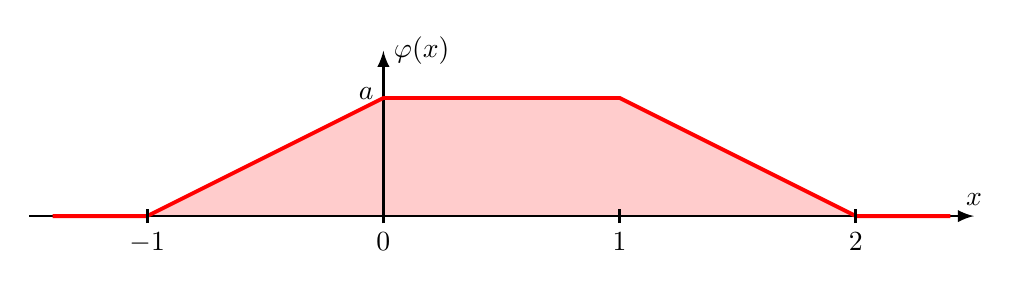
\begin{tikzpicture}[>=latex,scale=3]
\fill[color=red!20] (-1,0)--(2,0)--(1,0.5)--(0,0.5)--cycle;
\draw[->,line width=1pt] (-1.5,0)--(2.5,0)
	coordinate[label={$x$}];
\draw[->,line width=1pt] (0,-0.03)--(0,0.7)
	coordinate[label={right:$\varphi(x)$}];
\node at (0,0.52) [left] {$a$};
\draw[color=red,line width=1.4pt]
	(-1.4,0)--(-1,0)--(0,0.5)--(1,0.5)--(2,0)--(2.4,0);
\foreach \x in {-1,0,...,2}{
\draw[line width=1pt] ({\x},-0.03)--({\x},0.03);
\node at ({\x},-0.03) [below] {$\x$};
};
\end{tikzpicture}
\end{center}

\begin{loesung}
\begin{teilaufgaben}
\item Die Verteilung ist symmetrisch um den Wert $\mu=0.5$,
daher ist $E(X)=0.5$.
\item $a$ muss so gewählt werden, dass die rosarote Fläche eine Einheit ist.
Das Dreieck mit Ecken $(-1,0)$, $(0,0)$ und $(0,a)$ hat Grundseite $1$ und
Höhe $a$, also ist der Flächeninhalt $\frac{a}2$.
Dasselbe gilt für das Dreieck mit den Ecken $(1,0)$, $(2,0)$ und $(1,a)$.
Die Gesamtfläche unter der Kurve ist daher $2a$.
Sie wird $1$ genau dann, wenn man $a=\frac12$ wählt.
\item
Um die Varianz zu berechnen, muss $E(X^2)$ bestimmt werden.
\begin{align*}
E(X^2)
&=
\int_{-\infty}^\infty x^2 \varphi(x)\,dx
=
\int_{-1}^0 x^2 a(x+1)\,dx
+
\int_0^1 x^2a\,dx
+
\int_1^2 x^2a(2-x)\,dx
\\
&=
\frac12\biggl[
\frac{x^4}4+\frac{x^3}3
\biggr]_{-1}^0
+
\frac12\biggl[
\frac{x^3}3
\biggr]_{0}^1
+
\frac12\biggl[
\frac{2x^3}3
-
\frac{x^4}4
\biggr]_{1}^2
\\
&=
-\frac12\cdot\biggl(\frac14-\frac13\biggr)
+
\frac12\cdot\frac13
+
\frac12\cdot\biggl(\frac{16}3-\frac{16}4-\frac23+\frac14\biggr)
\\
&=
\frac1{24}
+\frac4{24}
+\frac{64-48-8+3}{24}
=
\frac1{24}
+\frac4{24}
+\frac{11}{24}
=
\frac{16}{24}
=
\frac{2}{3}.
\end{align*}
Daraus kann man jetzt die Varianz berechnen mit Hilfe von
\begin{align*}
\operatorname{var}(X)
&=
E(X^2) - E(X)^2
=
\frac{2}{3} - \frac{1}{4}
=
\frac{8-3}{12}=\frac{5}{12}=0.41666
\\
\sqrt{\operatorname{var}(X)}
&=
0.6455.
\qedhere
\end{align*}
\end{teilaufgaben}
\end{loesung}
